\documentclass{scrartcl}
\usepackage[latin1]{inputenc}
\usepackage[T1]{fontenc}
\usepackage[ngerman]{babel}
\usepackage{amsmath}
\usepackage{amssymb}
\usepackage{icomma}
%\usepackage[dvips]{graphicx}
%\usepackage{floatflt}
%\usepackage{enumitem}
%\usepackage{babel}
\usepackage{blindtext}
%\usepackage{showframe}
\usepackage{calc}
\usepackage{wrapfig}
\def\BILD{\rule{0.4\textwidth}{4cm}}

\usepackage{graphicx}
\usepackage{placeins}
\usepackage{multirow}
\usepackage{subfig}
\usepackage{url}

\renewcommand{\topfraction}{.85}
\renewcommand{\bottomfraction}{.7}
\renewcommand{\textfraction}{.15}
\renewcommand{\floatpagefraction}{.66}
\renewcommand{\dbltopfraction}{.66}
\renewcommand{\dblfloatpagefraction}{.66}
\setcounter{topnumber}{9}
\setcounter{bottomnumber}{9}
\setcounter{totalnumber}{20}
\setcounter{dbltopnumber}{9}
\setlength{\intextsep}{0cm plus1cm minus1cm}
\pdfminorversion = 5
\usepackage{setspace}
\onehalfspacing

\begin{document}
\title{Versuch 5: Millikan-Versuch}


\date{01.11.2010}


\author{Gruppe 5a: Gia-Danh Lam, Nils Haldenwang}

\maketitle
\tableofcontents

\section{Einleitung}
Elektrische Ladungen treten nur in gequantelten Werten als Vielfache
$n \cdot e$ der Elementarladung $e$ auf mit $ n \in \mathbb{Z}$. Im
Jahr 1910 gelang es Robert Andrews Millikan die Elementarladung $e$
relativ genau zu bestimmen, er erhielt $ e = 1.592 \cdot 10^{-19}C$
und daf�r sp�ter auch einen Nobelpreis. Nach heutigem Kenntnisstand
betr�gt der Wert $ e = 1,602 176 487 (40) \cdot 10^{-19} C$. Millikan
ist nicht der alleinige Erfinder des nach ihm benannten Versuches, er
griff auf vorherige Arbeiten von Harold Albert Wilson und Joseph John
Thomson zur�ck und verbesserte diese ma�geblich.

Zum Messen der Elementarladung werden �ltr�pfchen in einen
Kondensator, dessen Feld parallel zum Gravitationsfeld der Erde
ausgerichtet ist gebracht. Die untersuchten Tr�pfchen tragen nur einige wenige
Elementarladungen. Legt man keine Spannung an den Kondensator an, so
fallen die Tropfen mit einer konstanten Geschwindigkeit nach unten. Da
sie also offenbar nicht mehr beschleunigt werden, muss ein
Gleichgewicht der wirkenden Kr�fte vorliegen. Die wirkenden Kr�fte
sind in diesem Fall die Schwerkraft $F_g$, die Auftriebskraft $F_a$ und die
Reibungskraft $F_R$.

Schaltet man nun den Kondensator ein, so kommt die elektrostatische
Kraft $F_e$ des elektrischen Feldes auf das Tr�pfchen hinzu. Die
Richtung von $F_e$ ist je nach Polung unterschiedlich und ist somit
leicht umkehrbar. Nat�rlich �ndert sich mit der Bewegungsrichtung des
Tr�pfchens auch die Richtung der Reibungskraft $F_R$.

Der Aufbau und die Kr�fte sind schematisch in Abb. \ref{fig: Kraefte}
dargestellt.

\begin{figure}%[htb!]
\centering
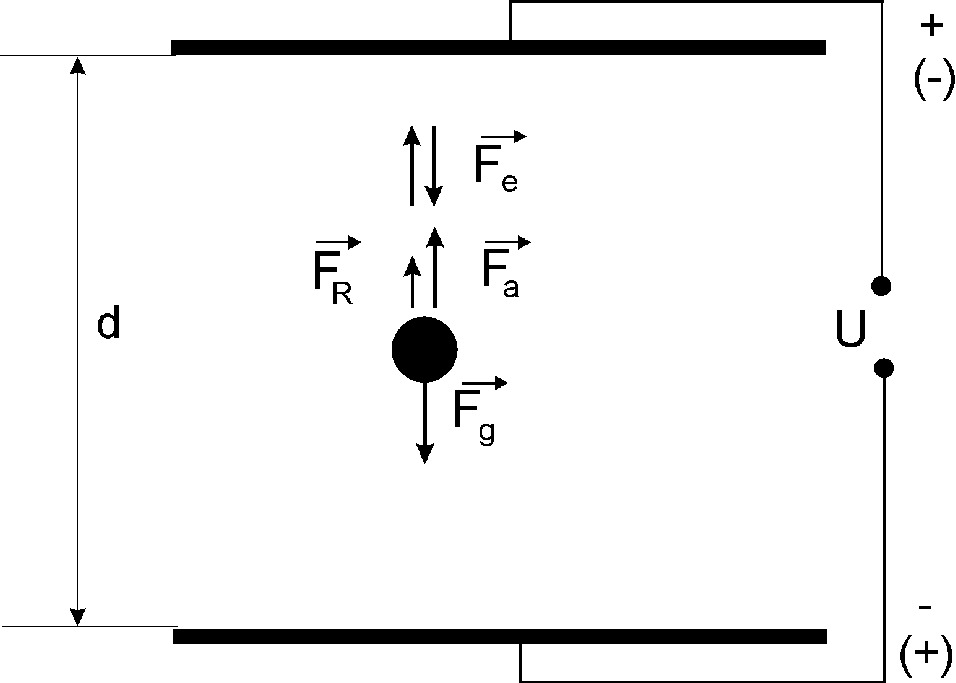
\includegraphics[width=12cm]{pics/SchemaAufbau}%
\caption{Schematischer Aufbau des Versuchs mit den wirkenden Kr�ften.}%
\label{fig: Kraefte}%
\end{figure}

\end{document}
